The Mini Wheelbot needs to be small, rigid, and powerful for learning experiments.
In this section, we summarize the custom design of hardware and electronics that is necessary to achieve these design goals and meet the specifications listed in Tab.~\ref{tab:robot_specs}.
\begin{table}[hbt]
    \caption{Specifications of the Mini Wheelbot.}
    \centering
    \begin{tabular}{|l|l|}
    \hline
    \textbf{Spec.} & \textbf{Value} \\
    \hline
    \hline
    Dims. & \SI{130}{\milli\meter} (height) x \SI{87}{\milli\meter} (width) \\
    \hline
    Weight & Total \SI{0.69}{\kilo\gram}, wheels \SI{0.13}{\kilo\gram} (each), body \SI{0.43}{\kilo\gram} \\
    \hline
    Motors & T-Motor MN4006, max.~\num{8000}~rpm, \SI{0.5}{\newton\meter} \\
    \hline
    Battery & \SI{450}{\milli\ampere\hour}, \SI{22.2}{\volt}, 6S LiPo, max. cont. \SI{20}{\ampere} discharge  \\
    \hline
    Runtime & \SI{45}{\minute} when balancing\\
    \hline
    CPU & Pi CM4, BCM2711 quad-core Cortex-A72, \SI{1.5}{\giga\hertz} \\
    \hline
    Sensors & 4x Bosch BMI088 IMU, 2x AMS AS5047D 14bit encoder\\
    \hline
    System & RT-Preempt Linux, Buildroot \\
    \hline
    \end{tabular}
    \label{tab:robot_specs}
\end{table}

\subsection{Mechanical Design}

\begin{figure}[tb]
    \centering
    \begin{table*}[ht]
    \centering
    
    \begin{subtable}{\linewidth}
        \centering
        \small
        \setlength{\tabcolsep}{8pt}
        \scalebox{0.9}[0.9]{
        \begin{tabular}{l*{7}c}
            \toprule
            {Method} & ImageNet & ImageNet-A & ImageNet-V2 & ImageNet-R & ImageNet-S & \textit{Average} & \textit{OOD Average} \\
            \midrule
            Baseline & 69.04 & 60.04 & 64.54 & 80.16 & 49.39 & 64.63 & 63.53 \\
            \textbf{+SOBA~(Ours)} & \textbf{70.90} & \textbf{61.06} & \textbf{65.83} & \textbf{80.79} & \textbf{52.57} & \textbf{66.23} & \textbf{65.06} \\
            \midrule
            \rowcolor{gray!30} Improvement & \textbf{+1.86} & \textbf{+1.02} & \textbf{+1.29} & \textbf{+0.63} & \textbf{+3.18} & \textbf{+1.60} & \textbf{+1.53} \\
            \bottomrule
        \end{tabular}}
        \caption{{Performance improvement of our method over cache baseline on OOD benchmark.}} 
    \end{subtable}
    
    \begin{subtable}{\linewidth}
        \centering
        \small
        \resizebox{\linewidth}{!}{
        \begin{tabular}{l*{11}c}
            \toprule
            Method & Aircraft & Caltech101 & Cars & DTD & EuroSAT & Flower102 & Food101 & Pets & SUN397 & UCF101 & \textit{Average} \\
            \midrule
            Baseline & 24.72 & 94.07 & 67.79 & 45.80 & 55.06 & 71.15 & 86.4 & 88.41 & 67.69 & 70.24 & 67.13 \\
            \textbf{+SOBA~(Ours)} & \textbf{25.62} & \textbf{94.60} & \textbf{71.12} & \textbf{46.87} & \textbf{59.44} & \textbf{71.66} & \textbf{86.69} & \textbf{92.48} & \textbf{70.63} & \textbf{74.12} & \textbf{69.32} \\
            \midrule
            \rowcolor{gray!30} Improvement & \textbf{+0.90} & \textbf{+0.53} & \textbf{+3.33} & \textbf{+1.07} & \textbf{+4.38} & \textbf{+0.51} & \textbf{+0.29} & \textbf{+4.07} & \textbf{+2.94} & \textbf{+3.88} & \textbf{+2.19} \\
            \bottomrule
        \end{tabular}
        }
        \caption{Performance improvement of our method over cache baseline on Cross-Dataset benchmark.} 
    \end{subtable}
    \vspace{-2mm}
    %实验以ViT-B/16为backbone。与baseline相比,我们的方法在所有数据集上的表现均有所提升。
    \label{tab:components}
    \caption{\textbf{Performance improvement of our method over cache baseline on both benchmarks.} The experiments employ ViT-B/16 as the backbone. Compared to the baseline, our method exhibits improved performance across all datasets.}
\end{table*}


    \caption{System overview of the Mini Wheelbot.}
    \label{fig:packaging}
\end{figure}

The Mini Wheelbot is designed to be compact, rugged, and powerful.
Its size is determined by the onboard compute module (a Raspberry Pi CM4) and six battery cells.
Brass is chosen as material for the reaction wheels due to its high density and good availability at CNC job shops.
Sizing calculations of the reaction wheels were performed as described in~\cite{geist2022wheelbot} to maximize rotational inertia needed for the stand-up maneuvers.
The body is made from aluminum, which is lightweight, durable, and inexpensive to machine.
Inside the body, compute module, battery pack, and power electronics are packed tightly (see Fig.~\ref{fig:packaging}).
The packaging minimizes body mass and inertia for highly dynamic maneuvers like stand-up and flips while keeping symmetry.

\subsection{Electronics Design}
The custom electronics inside the Mini Wheelbot are designed to maximize the robots power and control performance while ensuring safety and battery runtime.
An overview of custom electronics is shown in Fig.~\ref{fig:electronicsschematic}.
Schematics for all components are available online\footnote{\label{footnote:code}\codelink}.

\begin{figure}[b]
    \centering
    \begin{subfigure}[b]{3.4in}
        \centering
        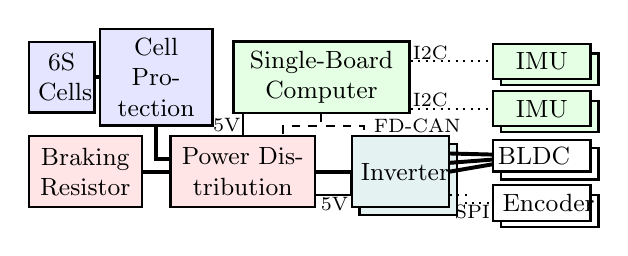
\begin{tikzpicture}[scale=1]   

    \node [rectangle, thick, draw, align=center, fill=blue!10, minimum height = 0.9cm, text width=0.6cm, font={\small}] (Cells) at (-1.5,1.2) 
    {6S Cells};

    \node [rectangle, thick, draw, align=center, fill=blue!10, minimum height = 0.9cm, text width=1.2cm, font={\small}] (BatteryProt) at (-0.3,1.2) 
    {Cell Protection};

    \node [rectangle, thick, draw, align=center, fill=red!10, minimum height = 0.9cm, text width=1.6cm, font={\small}] (PowerDistro) at (0.8,0)
    {Power Distribution};
    \node [rectangle, thick, draw, align=center, fill=red!10, minimum height = 0.9cm, text width=1.2cm, font={\small}] (BrakingResistor) at (-1.2,0)
    {Braking Resistor};
    
    \node [rectangle, thick, draw, align=center, fill=teal!10, minimum height = 0.9cm, text width=1cm, font={\small}] (InverterShadow) at (2.9,-0.1){};
    \node [rectangle, thick, draw, align=center, fill=teal!10, minimum height = 0.9cm, text width=1cm, font={\small}] (Inverter) at (2.8,0)
    {Inverter};

    \node [rectangle, thick, draw, align=center, fill=white, minimum height = 0.4cm, text width=1cm, align=center, font={\small}] (BLDCShadow) at (4.7,0.1)
    {};
    \node [rectangle, thick, draw, align=center, fill=white, minimum height = 0.4cm, text width=1cm, align=center, font={\small}] (BLDC) at (4.6,0.2)
    {};
    \node[align=center, font={\small}] at (4.5, 0.2) {BLDC};

    \node [rectangle, thick, draw, align=center, fill=white, minimum height = 0.4cm, text width=1cm, align=center, font={\small}] (EncoderShadow) at (4.7,-0.5)
    {};
    \node [rectangle, thick, draw, align=center, fill=white, minimum height = 0.4cm, text width=1cm, align=center, font={\small}] (Encoder) at (4.6,-0.4)
    {Encoder};

    \node [rectangle, thick, draw, align=center, fill=green!10, minimum height = 0.9cm, text width=2cm, font={\small}] (SBC) at (1.8,1.2)
    {Single-Board Computer};
    
    \node [rectangle, thick, draw, align=center, fill=green!10, minimum height = 0.4cm, text width=1cm, font={\small}] (IMU1Shadow) at (4.7,0.7)
    {};
    \node [rectangle, thick, draw, align=center, fill=green!10, minimum height = 0.4cm, text width=1cm, font={\small}] (IMU1) at (4.6,0.8)
    {IMU};
    
    \node [rectangle, thick, draw, align=center, fill=green!10, minimum height = 0.4cm, text width=1cm, font={\small}] (IMU2Shadow) at (4.7,1.3)
    {};
    \node [rectangle, thick, draw, align=center, fill=green!10, minimum height = 0.4cm, text width=1cm, font={\small}] (IMU2) at (4.6,1.4)
    {IMU};

    \begin{scope}[
        every node/.style={rectangle, align=center, font={\scriptsize}},
        every edge/.style={thick, draw, line width = 0.25mm},
        every path/.style={thick, draw, line width = 0.25mm}
    ]

        \draw[dotted] (SBC.east)++(0,-0.4) |- node [above right=-0.1cm]{I2C} (IMU1.west);
        \draw[dotted] (SBC.east)++(0,0.2)  |- node [above right=-0.1cm]{I2C} (IMU2.west);
        \draw[dotted] (Inverter.-25) -| ++(0.2,0) |- (Encoder.west) node [below left=-0.1cm]{SPI} ;
        \draw[-] (SBC.south)++(-1,0) -- node [left=-0.1cm]{5V} (PowerDistro.north);
        \draw[dashed] (SBC.south)++(0,0) -- ++(0,-0.15) -| node [right]{FD-CAN} (Inverter.135);
        \draw[dashed] (SBC.south)++(0,0) -- ++(0,-0.15) -| (PowerDistro.42);
        \draw[-] (PowerDistro.east)++(0,-0.3) -| node [below left=-0.1cm]{5V}  (Inverter.west);
    \end{scope}
    
    \begin{scope}[
        every node/.style={rectangle, align=center, font={\scriptsize}},
        every edge/.style={very thick, draw, line width = 0.5mm},
        every path/.style={very thick, draw, line width = 0.5mm}
    ]
        \draw[-] (Cells) -- (BatteryProt);
        \draw[-] (BatteryProt.south) |- (PowerDistro.170);
        \draw[-] (PowerDistro.west) -- (BrakingResistor.east);
        \draw[-] (PowerDistro) -- (Inverter);
        \draw[-] (Inverter.20) --  (BLDC);
        \draw[-] (Inverter.10)  --  (BLDC);
        \draw[-] (Inverter.0) -- (BLDC);
    \end{scope}

\end{tikzpicture}

    \end{subfigure}
    \par\medskip %
    \begin{subfigure}[b]{3.4in}
        \centering
        \newcommand{\photoheight}{0.64in}
        \begin{tikzpicture}
    \node[anchor=south west,inner sep=0] (img1) at (0,0) {\includegraphics[height=\photoheight]{figures/electronics/photos/battery_parts.jpg}};
    
    \node[anchor=south west,inner sep=0] (img2) at (img1.south east){\includegraphics[height=\photoheight]{figures/electronics/photos/battery_complete.jpg}};

    \begin{scope}[
        x={($0.1*(img1.south east)$)},
        y={($0.1*(img1.north west)$)}]
        \draw[latex-, thin, black, black] (2.4,3.0) -- (2.4,1.15)
        node[black,anchor=north,font=\tiny, inner sep=0.6, text=black, fill=white, fill opacity=0.5, text opacity=1, rounded corners=0.8](label){Cells};
        \draw[latex-, thin, black] (5.2,1.7) -- (label.east);

        \draw[latex-, thin,black, black] (4.7,8.7) -- (3,8)
        node[black,anchor=north,font=\tiny, inner sep=0.6, text=black, fill=white, fill opacity=0.5, text opacity=1, rounded corners=0.8]{Protection};


        
    
    \end{scope}
    \node[overlay, font=\tiny,  anchor=south east, text width = 0.365in, align = right, yshift=0.5mm, xshift=-0.5mm, inner sep=0.8, text=black, fill=white, fill opacity=0.5, text opacity=1, rounded corners=0.8] at (img2.south east) {Assembled Battery Pack};
\end{tikzpicture}
%
        \begin{tikzpicture}
    \node[anchor=south west,inner sep=0] (img1) at (0,0) {\includegraphics[height=\photoheight]{figures/electronics/photos/power_distribution.jpg}};
    
    \begin{scope}[
        x={($0.1*(img1.south east)$)},
        y={($0.1*(img1.north west)$)}]
        \node[overlay, black,anchor=north,font=\tiny, inner sep=0.4, text=black, fill=white, fill opacity=0.5, text opacity=1, rounded corners=0.8] (braking_resistor) at (3.1,1.2) {Braking Resistor};
        \draw[latex-, thin,black, black] (1.8,3.5) -- ($(braking_resistor.north) + (-15pt,0)$); 

        
    
        \node[overlay, font=\tiny, inner sep=0.6, text=black, fill=white, fill opacity=0.5, text opacity=1, rounded corners=0.8] at (5,9.4) {Power Distribution};
    \end{scope}
\end{tikzpicture}
%
        \begin{tikzpicture}
    \node[anchor=south west,inner sep=0] (img1) at (0,0) {\includegraphics[height=\photoheight]{figures/electronics/photos/compute_imu.jpg}};
    
    \begin{scope}[
        x={($0.1*(img1.south east)$)},
        y={($0.1*(img1.north west)$)}]
        \draw[latex-, thin,black, black] (2.8,3.5) -- (2.3,1.02)
        node[black,anchor=north,font=\tiny, inner sep=0.4, text=black, fill=white, fill opacity=0.5, text opacity=1, rounded corners=0.8] (label) {IMU};
        \draw[latex-, thin,black, black] (6,1.2) -- (label.north);

        \draw[latex-, thin,black, black] (2.5,9.3) -- (5.5,9.45)
        node[black,anchor=west,font=\tiny, inner sep=0.4, text=black, fill=white, fill opacity=0.5, text opacity=1, rounded corners=0.8] (label2) {IMU};
        \draw[latex-, thin,black, black] (7.2,7.5) -- (label2.south);

        
    
    \end{scope}
\end{tikzpicture}
%
        \begin{tikzpicture}
    \node[anchor=south west,inner sep=0] (img1) at (0,0) {\includegraphics[height=\photoheight]{figures/electronics/photos/inverter.jpg}};
    \node[overlay, font=\tiny,  anchor=north east, align = right, yshift=-0.25mm, xshift=-0.25mm, inner sep=0.8, text=black, fill=white, fill opacity=0.5, text opacity=1, rounded corners=0.8] at (img1.north east) {Inverters};
\end{tikzpicture}
%
    \end{subfigure}
    \caption{Electronics design of the Mini Wheelbot (top) and custom circuit boards (bottom).}
    \label{fig:electronicsschematic}
\end{figure}

The removable battery pack has six \SI{450}{\milli\ampere\hour} Lithium Polymer cells (three on each side of the robot) protected by two BQ77915 with overcurrent and short-circuit protection -- all safely potted in one housing (Fig.~\ref{fig:electronicsschematic}, bottom left).
The power distribution board monitores power consumption and engages a braking resistor in case recuperated current during stand-up maneuvers can not be charged back into battery or external power supply.
In addition, a~nRF24L01P communicates with a wireless emergency stop button to shut off motor controllers.
Two custom inverters based on the $\mu$Motor~\cite{lehmann2021micro} run field-oriented control (FOC) to drive T-Motor MN4006 brushless DC motors.
Current is measured low-side on all phases at FOC loop frequency of~\SI{40}{\kilo\hertz}.
Due to careful analog design and INA241A2 current sense amplifiers, the gains of the PI d-q-current controllers can be chosen as high as~\SI{10}{\kilo\hertz} bandwidth.
On-axis magnetic 14-bit AS5047 encoders are interfaced by the inverters via SPI with transfers triggered from an interrupt synchronized with the FOC loop.
The motors exhibit strong cogging with peaks of up to~\SI{20}{\milli\newton\meter} (\SI{4}{\percent} of the maximum torque).
This severely impacts balancing control.
We therefore implement cogging compensation with a lookup table of feedforward torques.
These are calibrated by sweeping through a full rotation in \num{4000} steps with a high-gain position controller and saving the average current to hold each position in flash memory on the inverter (cf.~\cite{piccoli2016anticogging} for details).
The compensation effectively reduces the cogging to less than~\SI{2.5}{\milli\newton\meter} (\SI{0.5}{\percent}).
Power distribution and inverters are commanded via CAN-FD with an MCP2517FD controller by the Raspberry Pi CM4 compute module at~\SI{1}{\kilo\hertz}.
Bosch BMI088 IMUs are directly interfaced via I2C from the CM4.

\subsection{Software}
The Mini Wheelbot runs a Buildroot Linux with real-time kernel.
The single-board computer performs all higher-level estimation and control, implemented in C++ and running inside a Docker container.
While sending CAN messages through Linux SocketCAN is almost latency free in this setup, there is significant delay (up to~\SI{10}{\milli\second}) between the kernel interrupt and receiving encoder values on the user-space socket.
This delay is due to the processing of received CAN messages by the same workers as all other networking and can be compensated in software by extrapolation.
IMUs readings are available through the Linux IIO subsystem.
